\textbf{ID:} UC06 (Delete Event) \\
\textbf{Scope:} CS Automated Information Timeline \\
\textbf{Level:} User Goal \\
\textbf{Primary Actor:} Faculty \\
\textbf{Stakeholders and Interests:}
\begin{itemize}
    \item Audience: Wants to view up-to-date information about events in the CS Department
    \item Faculty: Wants the ability to delete events that they submitted that are no longer happening
    \item Office Manager: Wants to display accurate event information on the calendar on the Lobby TV
\end{itemize}
\textbf{Preconditions:} Faculty created an event (UC04) and submitted it for review (UC08). Admin/Reviewer reviewed the event (UC09) and approved. Faculty is identified and authenticated in the system and is viewing the event calendar (UC03). \\
\textbf{Postconditions:} Event status is in a deleted state. \\
\textbf{Main Success Scenario:}
\begin{enumerate}
    \item Faculty clicks the ``View My Events'' link on the event calendar page.
    \item System returns a list of existing events authored by Faculty that have been approved.
    \item Faculty selects the event they wish to delete from the returned list of their previously approved events.
    \item System returns the event page for the selected event.
    \item Faculty clicks the ``Delete This Event'' button on the event page.
    \item System prompts Faculty to confirm the removal of the event from the event calendar.
    \item Faculty confirms the removal of the event from the event calendar by clicking ``Yes''.
    \item System provides Faculty with a confirmation message.
\end{enumerate}
\textbf{Extensions (or Alternate Flows):} \\
3a. Faculty does not see the event they wish to delete in the returned list because the event has not yet been approved by the Admin/Reviewer:
\begin{enumerate}
    \item Faculty must wait for approval from Admin/Reviewer on the original event before the event is eligible for removal from the event calendar.
\end{enumerate}
7a. Faculty decides they do not want to remove the event from the event calendar:
\begin{enumerate}
    \item Faculty clicks the ``No'' button and is redirected to the list of existing events authored by Faculty that have been approved.
\end{enumerate}
\textbf{Special Requirements:} None \\
\textbf{Technology and Data Variations List:} None \\
\textbf{Frequency of Occurrence:} Maximum once per submitted and approved event. \\
\textbf{Open Issues:} None \\

\begin{figure}[H]
    \centering
    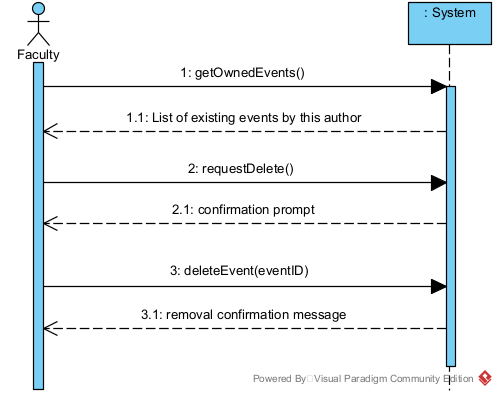
\includegraphics[width=0.8\textwidth]{images/SSD-UC06-DeleteEvent.png}
    \centering
    \caption{System Sequence Diagram: Delete Event}
\end{figure}

\textbf{Operation:} requestDelete() \\
\textbf{Cross-References:} UC06 (Delete Event) \\
\textbf{Pre-conditions:}
\begin{itemize}
    \item Event object has been created.
    \item Event attribute status is set to approved.
    \item Event has been associated with Faculty.
\end{itemize}
\textbf{Post-conditions:} None \\

\textbf{Operation:} deleteEvent(eventID) \\
\textbf{Cross-References:} UC06 (Delete Event) \\
\textbf{Pre-conditions:}
\begin{itemize}
    \item Event object has been created.
    \item Event attribute status is set to approved.
    \item Event has been associated with Faculty.
\end{itemize}
\textbf{Post-conditions:}
\begin{itemize}
    \item Event attribute status is set to deleted.
    \item Event associated with Faculty has been broken.
\end{itemize}